\documentclass[10pt,twocolumn,letterpaper]{article}

\usepackage{cvpr}
\usepackage{times}
\usepackage{epsfig}
\usepackage{graphicx}
\usepackage{amsmath}
\usepackage{ulem}
\usepackage{amssymb}

% Include other packages here, before hyperref.
\DeclareMathOperator*{\E}{\mathbb{E}}


% If you comment hyperref and then uncomment it, you should delete
% egpaper.aux before re-running latex.  (Or just hit 'q' on the first latex
% run, let it finish, and you should be clear).
\usepackage[breaklinks=true,bookmarks=false]{hyperref}

\cvprfinalcopy % *** Uncomment this line for the final submission

\def\cvprPaperID{****} % *** Enter the CVPR Paper ID here
\def\httilde{\mbox{\tt\raisebox{-.5ex}{\symbol{126}}}}

% Pages are numbered in submission mode, and unnumbered in camera-ready
%\ifcvprfinal\pagestyle{empty}\fi
\setcounter{page}{1}
\let\svthefootnote\thefootnote
\begin{document}

%%%%%%%%% TITLE
\title{LOGAN-B : Bidirectional Latent Optimized Generative Adversarial Networks}

\author{Sharath Ramkumar\\
University of Massachusetts, Amherst\\
{\tt\small sharathramku@cs.umass.edu}
} 

\maketitle
%\thispagestyle{empty}

%%%%%%%%% ABSTRACT
\begin{abstract}
    The inductive bias of generative adversarial networks is a powerful tool for learning distributions of data. However, these models are difficult to train and very susceptible to mode collapse, capturing only a few modes of the data distribution. In this work, we introduce bidirectional latent optimized generative adversarial networks as a framework for training generative adversarial networks to mitigate this problem by encouraging the generator to maintain a mapping to the data distribution.
\end{abstract}


\let\thefootnote\relax\footnote{All code will be available at \href{https://github.com/sharath/logan-b}{github.com/sharath/logan-b}.}
\addtocounter{footnote}{-1}\let\thefootnote\svthefootnote

%%%%%%%%% BODY TEXT
\section{Introduction}

Generative Adversarial Networks (GANs) are a class of generative models that learn a data distributions. GANs have achieved impressive results on various computer vision tasks such as image generation \cite{karras2017progressive, brock2018large, karras2019analyzing}, style transfer \cite{zhu2017unpaired, zhu2017toward, isola2017image}, and domain adaptation \cite{tzeng2017adversarial, su2019active, sankaranarayanan2018generate} among others. However, GANs are still notoriously difficult to train without careful hyperparameter tuning and susceptible to mode collapse.

\subsection{Motivation}

The optimal generator in the GAN setup can be seen as an approximation of the training data. In fact, in \cite{goodfellow2014generative}, Goodfellow et al. show that the optimal generator has the same distribution of data samples as the training data. If this is actually true, then it should be possible to sample the training data from the implicit distribution defined by the generator. However, the generator training process is unstable and susceptible to mode collapse, often losing its capability to generate diverse samples. By forcing the generator to maintain a mapping, we hope to encourage the generator to generate diverse samples.


\subsection{Related Work}

\subsubsection{LOGAN: Latent Optimization for GANs}

Very recently, Wu et al. introduced a similar form of latent optimization in \cite{wu2019logan} where the latent space is jointly optimized with the generator and discriminator. They use the natural gradient \cite{amari1998natural} to optimize the latent and show that it results in better IS/FID scores on BigGAN \cite{brock2018large}. This definition of latent optimization differs from the one defined by \cite{bojanowski2017optimizing}, which is the focus of this work.

\subsubsection{EBGAN: Energy-based GANs}

In \cite{zhao2016energy}, Zhao et al. propose EBGAN, a GAN which uses an autoencoder in the discriminator network to encourage the generator network to produce images that contain features that can be used to reconstruct itself. This can be seen as a form of regularization to retain the training data in the generator's implicit distribution.

\subsection{Contributions}

Our contributions are as follows:
\begin{itemize}
    \item We introduce latent optimization for an encoder in a bi-directional generative adversarial network using a surrogate reconstruction loss.
    \item We show that our framework captures the space of the true distribution more accurately than the GAN \cite{goodfellow2014generative} baseline on a synthetic dataset.
    \item We show that our framework stabilizes post hoc \cite{dumoulin2016adversarially} reconstructions on MNIST and CIFAR10.
\end{itemize}


%-------------------------------------------------------------------------
\section{Background}

This section provides a background on GANs, latent optimization, and latent space image embedding.

\subsection{Generative Adversarial Networks}

GANs were introduced in \cite{goodfellow2014generative} by Goodfellow et al. In the GAN setting, we wish to find a discriminator $D$ and a generator $G$ that satisfy a mini-max game for a data distribution $p_{\mathcal{X}}$ and a prior distribution $p_{\mathcal{Z}}$. In practice, we represent $G$ and $D$ using neural networks and we optimize the parameters of the networks in a joint manner alternating between each network, in a manner that can be seen as two players taking turns:

\begin{equation}
    \min_{G}\max_{D} \E_{x \sim p_{\mathcal{X}}}\left[\log(D(x))\right] + \E_{z \sim p_{\mathcal{Z}}}\left[\log(1 - D(G(z)))\right].
    \label{eq:gan_opt}
\end{equation}

\subsection{Generative Latent Optimization}

The generative latent optimization (GLO) framework was proposed by Bojanowski et al. in \cite{bojanowski2017optimizing}. For a large set of images, $\{x_i\}_{i=1}^N$, with each image $x_i \in \mathcal{X}$, we assign a $d$-dimensional vector $z_i \in \mathcal{Z}$ to each image. Then perform a joint optimization of the parameters of the generator network and the noise vector for the input to the network:

\begin{equation}
    \min_{G} \frac{1}{N}\sum_{i=1}^{N}\left[\min_{z_i\in\mathcal{Z}} \ell(G(z_i), x_i) \right].
    \label{glo_opt}
\end{equation}

\subsection{Latent Space Embedding}

A variety of methods have been proposed to find latent embeddings for natural images in the Generator's latent space. In this work, we compare against the Bidirectional GAN (BiGAN) \cite{donahue2016bigan} and variants of optimization \cite{bau2019seeing} on the input. More formally, the latent space embedding $z$ of a natural image $x$ can be written as the following optimization problem:

\begin{equation}
    \min_{z\in\mathcal{Z}}{\ell(G(x), x)}.
    \label{embdding_opt}
\end{equation}

In (\ref{embdding_opt}), $\ell$ is a distance metric between two images. Possible choices for $\ell$ include L1/L2, perceptual distance \cite{zhang2018unreasonable}, and Laplacian pyramid loss \cite{ling2006diffusion} among others.

\subsubsection{Input Optimization}

One approach to obtaining an embedding for an image is by optimizing the input directly. Other variations of this include \textit{stochastic clipping} for priors with finite supports, proposed by Tripathi et al. in \cite{lipton2017precise} and layer-wise optimization proposed by Bau et al. in \cite{bau2019seeing}. In this approach, we initialize an input noise vector by sampling from the prior and then perform gradient descent on the input to minimize the distance metric.

\subsubsection{Bidirectional Generative Adversarial Networks (BiGANs)}

Another approach to obtain latent space image embeddings is to pass the natural image through an encoder network that is trained jointly with the the Generator. This jointly trained network is called an \textit{ad hoc encoder}. In the BiGAN framework, the generator and encoder are inverses of each other at the global optima \cite{donahue2016bigan, dumoulin2016adversarially}.  The optimization problem is framed as the following:

\begin{equation}
    \min_{G, E} \max_{D} \E_{x \sim p_{\mathcal{X}}}\left[\log(D(x, E(x)))\right] + \E_{z \sim p_{\mathcal{Z}}}\left[\log(1 - D(G(z), z))\right].
    \label{bigan_opt}
\end{equation}

\subsection{Performance Metrics}

This section provides an overview of the metrics we use to measure performance.

\subsubsection{Inception Score}

Inception score (IS) is a metric for evaluating the quality of samples from a generator \cite{salimans2016improved}. The score is calculated using features from the Inception network \cite{szegedy2016rethinking}. Salimans et al. found that that the IS metric is correlated with human evaluation. Higher values of IS correspond to a ``better'' generator network.

\subsubsection{Fréchet Inception Distance}

Fréchet Inception Distance (FID) is a distance metric proposed by Heusel et al. in \cite{heusel2017gans} as an improvement over the IS metric by using the statistics of the training dataset. The FID metric has also been shown to be more robust to disturbances to samples such as noise and occlusions. This is a distance metric, so lower values of FID correspond to a ``better'' generator network.

\subsubsection{Reconstruction Error} \label{recerror}

While IS and FID  are reasonable \cite{ravuri2019seeing} metrics for sample quality, we also report the average reconstruction error of an encoder trained after the generator. We refer to this as the \textit{post hoc} \cite{dumoulin2016adversarially} encoder, in contrast to the BiGAN encoder which is \textit{ad hoc}. We train an encoder network using the  latent random noise as the target and images from the generator as the input $5$ times. Then we compute the mean and standard deviation of the reconstruction losses on the holdout data and report that. Low values for reconstruction error indicate:
\begin{enumerate}
    \item the extent to which the generator captures the distribution of the training data
    \item and the invertibility of the generator, which can be seen as a measure of latent optimality.
\end{enumerate}

\section{Bidirectional Latent Optimized Generative Adversarial Network}

The bidirectional latent optimized GAN (LOGAN-B) jointly trains an encoder $E$, generator $G$, and discriminator $D$ with the following loss functions:

\begin{equation}
    \mathcal{L}_{G} = \E_{z \sim p_{\mathcal{Z}}}\left[\log(1 - D(G(z), z))\right] + \mathcal{L}_{S}
\end{equation}

\begin{equation}
    \mathcal{L}_{E} = \E_{x \sim p_{\mathcal{X}}}\left[\log(D(x, E(x)))\right] + \mathcal{L}_{S}
\end{equation}

\begin{equation}
    \mathcal{L}_{D} = - \E_{x \sim p_{\mathcal{X}}}\left[\log(D(x, E(x)))\right] - \E_{z \sim p_{\mathcal{Z}}}\left[\log(1 - D(G(z), z))\right]
\end{equation}

where $\mathcal{L}_{S}$ is the surrogate reconstruction loss:

\begin{equation}
    \mathcal{L}_{S} =  \E_{x\sim p_{\mathcal{X}}}\left[ \ell(x, G(E(x))) \right]
    \label{surrogate_loss}
\end{equation}

\begin{figure}
    \centering
    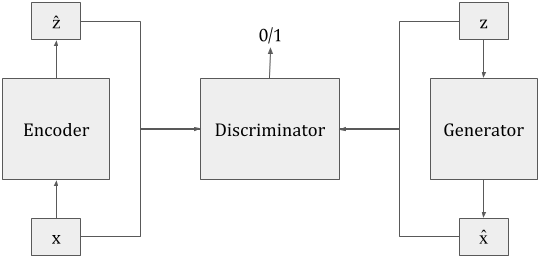
\includegraphics[width=\linewidth]{diagrams/bigan.png}
    \phantom{\;}
    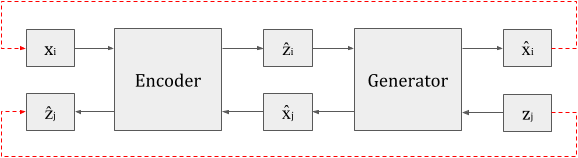
\includegraphics[width=\linewidth]{diagrams/surrogate.png}
    \caption{Overview of the adversarial and surrogate setup for LOGAN-B. First we update discriminator, generator, and encoder using adversarial losses. Then we update the encoder and generator using the surrogate reconstruction loss.}
    \label{fig:overview_diagram}
\end{figure}

\subsection{Relationship to BiGAN and GLO}

In the BiGAN framework, the optimal encoder is capable of inverting the optimal generator \cite{donahue2016bigan}.  This is a form of latent optimization as defined by Bojanowski et al. in  \cite{bojanowski2017optimizing}:

\begin{equation}
    \min_{G} \frac{1}{N}\sum_{i=1}^{N}\left[\min_{z_i\in\mathcal{Z}} \ell(x_i, G(z_i)) \right]
\end{equation}

\begin{equation}
    \min_{G, E} \frac{1}{N}\sum_{i=1}^{N}\left[ \ell(x_i, G(E(x_i))) \right]
    \label{glo_sum}
\end{equation}

\begin{equation}
    \approx \min_{G, E}  \E_{x\sim p_{\mathcal{X}}}\left[ \ell(x, G(E(x))) \right]
    \label{glo_expt}
\end{equation}

The problems defined by \eqref{glo_sum} and \eqref{glo_expt} are equal as $N$ approaches $\infty$ \cite{donahue2016bigan} . Under the same conditions, the optimal generator and encoder in the BiGAN framework also satisfy all of these optimization problems:

\begin{equation}
    \min_{G, E} \E_{x\sim p_{\mathcal{X}}}\left[ \ell(x, G(E(x))) \right]
    \label{rc_loss1}
\end{equation}

\begin{equation}
    \min_{G, E} \E_{x\sim p_{\mathcal{X}}}\left[ \ell(E(x), E(G(E(x)))) \right]
\end{equation}

\begin{equation}
    \min_{G, E} \E_{x\sim p_{\mathcal{X}}}\left[ \ell(x, G(E(G(E(x))))) \right]
    \label{rc_loss2}
\end{equation}

\begin{equation}
    \min_{G, E} \E_{x\sim p_{\mathcal{X}}}\left[ \ell(E(x), E(G(E(G(E(x)))))) \right]
\end{equation}

\begin{equation*}
    \dots
\end{equation*}

Under the same conditions, these are also all equivalent optimization problems over the latent space:

\begin{equation}
    \min_{G, E} \E_{z\sim p_{\mathcal{Z}}}\left[ \ell(z, E(G(z))) \right]
    \label{1storder_il}
\end{equation}

\begin{equation}
    \min_{G, E} \E_{z\sim p_{\mathcal{Z}}}\left[ \ell(G(z), G(E(G(z)))) \right]
    \label{1storder_rl}
\end{equation}

\begin{equation}
    \min_{G, E} \E_{z\sim p_{\mathcal{Z}}}\left[ \ell(z, E(G(E(G(z))))) \right]
\end{equation}

\begin{equation}
    \min_{G, E} \E_{z\sim p_{\mathcal{Z}}}\left[ \ell(G(z), G(E(G(E(G(z)))))) \right]
\end{equation}

\begin{equation}
    \min_{G, E} \E_{z\sim p_{\mathcal{Z}}}\left[ \ell(z, E(G(E(G(E(G(z))))))) \right]
\end{equation}

\begin{equation*}
    \dots
\end{equation*}

Donahue et al. propose \eqref{1storder_il} in \cite{donahue2016bigan} as the \textit{latent regressor}. They show that using \eqref{1storder_il} performs poorly since the generator is not actually optimal during training. Furthermore, they argue that this has limited benefits: Since the encoder never sees the training data, the loss biases the optimization towards a local optima near its current parameters rather than near the global minimum. To rectify this, we propose using samples from the training data to minimize \eqref{rc_loss1} as the \textit{surrogate loss}. We speculate that other combinations may contain useful gradients, but leave them to future work.

\section{Experiments}

\subsection{Synthetic Data}

We consider a synthetic dataset of $8$ Gaussian distributions and report the reconstruction error (as defined in \ref{recerror}) in Table \ref{tab:synthetic_err}. We use the L1 distance function for $\ell$ and a uniform noise distribution for the prior. Post hoc encoders are initialized randomly and trained to estimate the input to the generator that produced the samples. The ad hoc encoder for the GAN does not affect training, it is simply updated with the generator.

\begin{table}[!ht]
    \centering
    \begin{tabular}{lrr}
        Method & ad hoc & post hoc \\\hline
        GAN     & $2.7937$ & $0.1261 \pm 0.0060$ \\
        BiGAN   & $2.5036$ & $1.4310 \pm 0.0744$ \\
        LOGAN-B & $0.0271$ & $0.0474 \pm 0.0057$ \\
    \end{tabular}
    \caption{Ad hoc/post hoc reconstruction errors on the synthetic dataset.}
    \label{tab:synthetic_err}
\end{table}

\begin{figure*}
\begin{center}
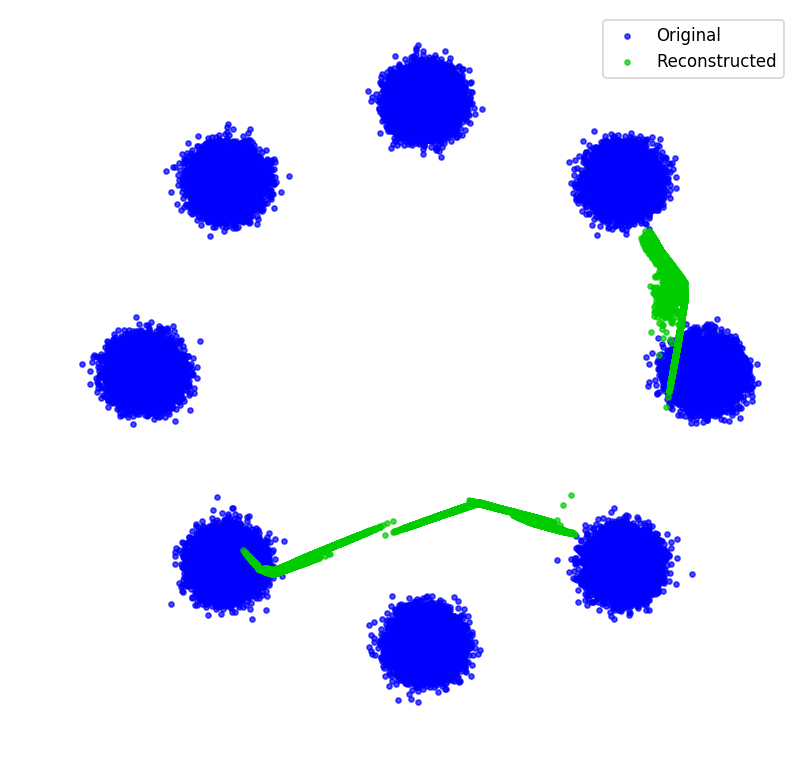
\includegraphics[width=0.3\linewidth]{synthetic/adhoc-gan.png}
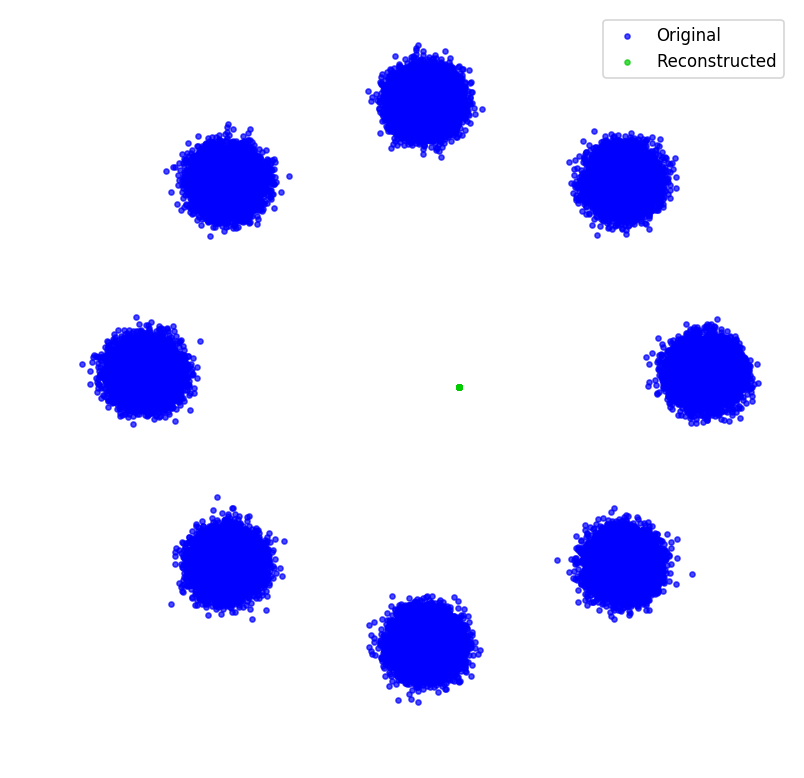
\includegraphics[width=0.3\linewidth]{synthetic/adhoc-bigan.png}
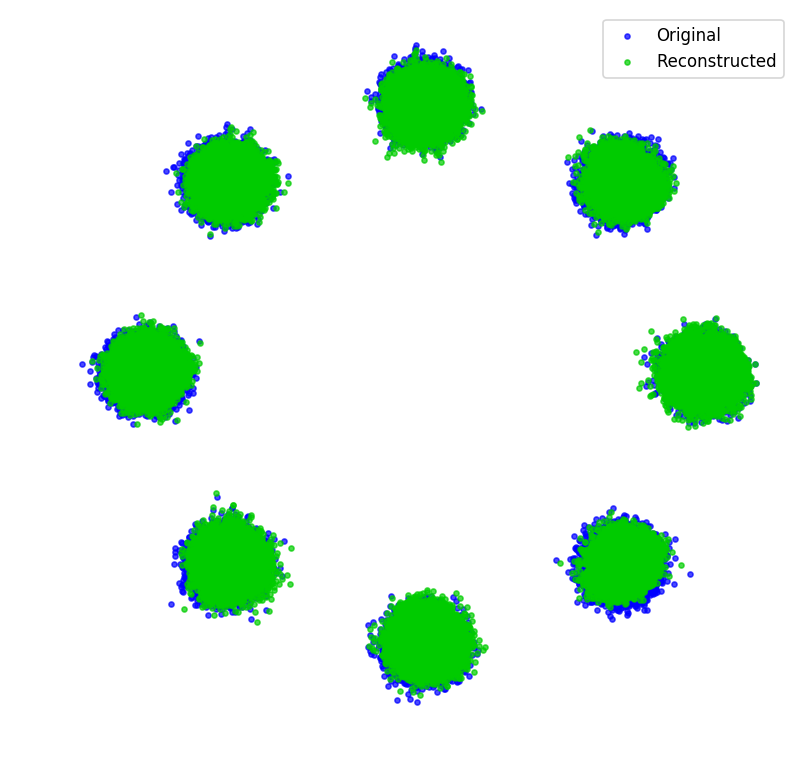
\includegraphics[width=0.3\linewidth]{synthetic/adhoc-logan-b.png}
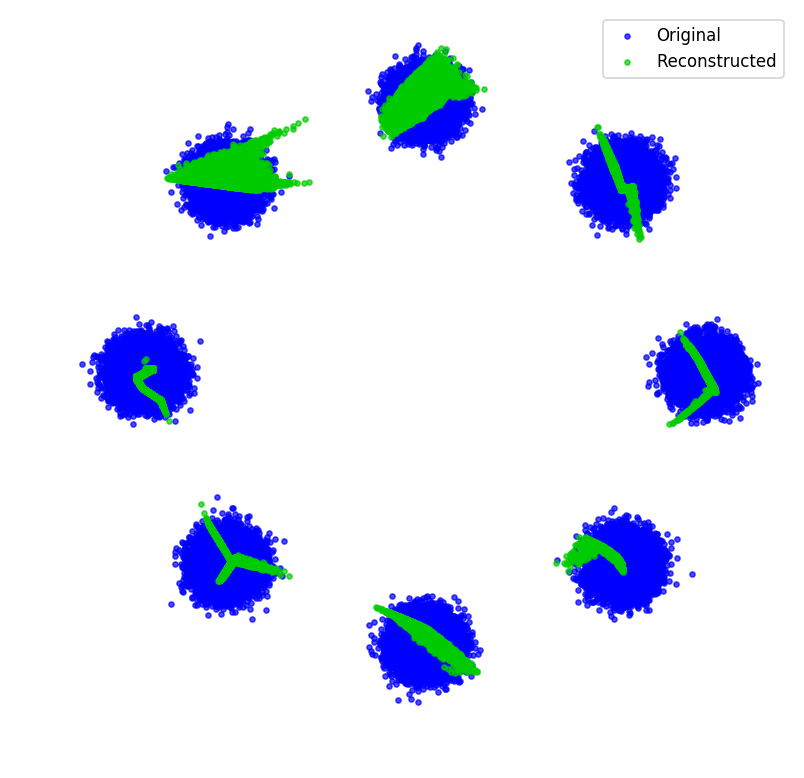
\includegraphics[width=0.3\linewidth]{synthetic/posthoc-gan.png}
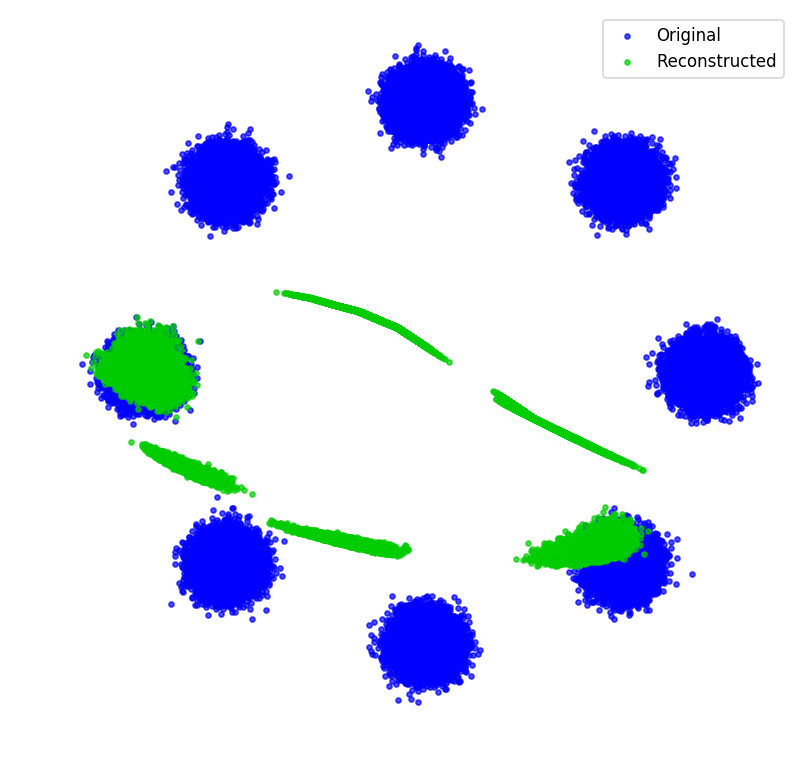
\includegraphics[width=0.3\linewidth]{synthetic/posthoc-bigan.png}
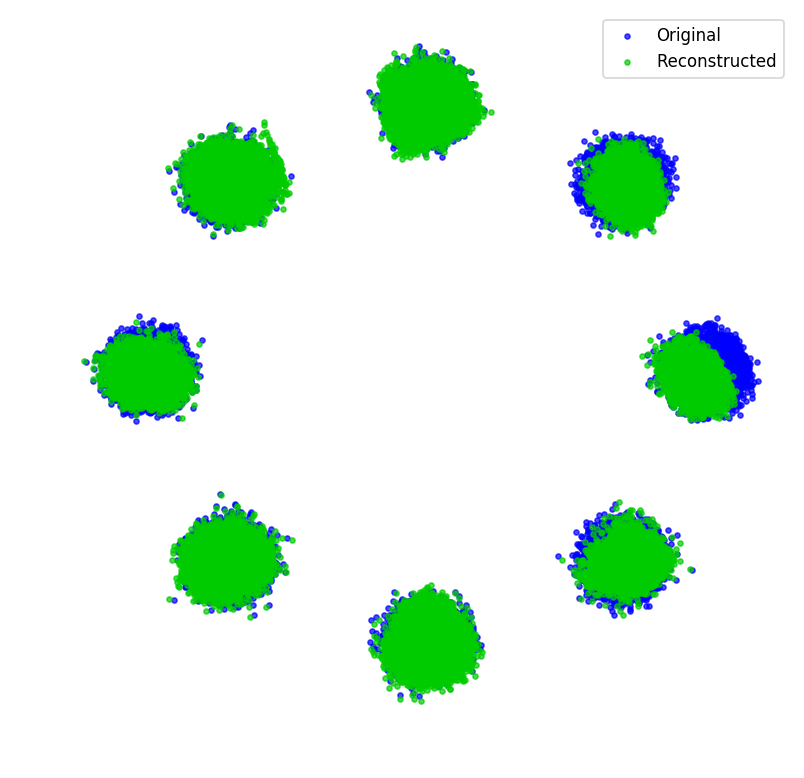
\includegraphics[width=0.3\linewidth]{synthetic/posthoc-logan-b.png}
\caption{Reconstructions on the synthetic Gaussian mixture dataset. Reconstructions for GAN, BiGAN, and LOGAN-B (left-to-right) for both ad hoc (top) and post hoc (bottom) trained encoders. The BiGAN ad hoc encoder collapsed, but the post hoc encoder shows a more accurate view of the performance of the BiGAN generator.}
\end{center}
\label{fig:recon_synthetic_fig}
\end{figure*}

The reconstructions (Figure \ref{fig:recon_synthetic_fig}) that the BiGAN encoder collapses to during training always map to the center of the ring. However, the post hoc encoder for the same generator network shows that the generator still maintains mappings from the latent space to some of the Gaussian distributions in the training data.

\subsection{MNIST}

For our experiments on the MNIST \cite{lecun1998gradient} dataset, we use LOGAN-B with the DCGAN \cite{radford2015unsupervised} architectures for the generator and discriminator and an inverted DCGAN generator for the encoder. MNIST images were resized to $32\times 32$ and normalized. Performance metrics were computed after the $10$th epoch. 

\begin{table}[!ht]
    \centering
    \begin{tabular}{lrrrr}
        Method & ad hoc & post hoc & IS & FID\\\hline
        DCGAN   & $290.82$ & $101.76 \pm 3.76$ & $2.13$ & $71.68$ \\
        BiGAN   & $720.15$ & $720.04 \pm 0.49$ & $1.00$ & $431.01$ \\
        LOGAN-B & $29.99$  &  $31.01 \pm 1.33$ & $2.01$ & $40.23$ \\
    \end{tabular}
    \caption{Ad hoc/post hoc reconstruction errors and IS/FID scores for MNIST. Lower FID is better. Higher IS is better.}
    \label{tab:mnist_err}
\end{table}


\subsection{CIFAR10}

For our experiments on the CIFAR10 \cite{krizhevsky2009learning} dataset, we use LOGAN-B with the DCGAN \cite{radford2015unsupervised} architectures for the generator and discriminator and a inverted generator for the encoder. CIFAR10 images were normalized. Performance metrics were computed after the $25$th epoch.

\begin{table}[!ht]
    \centering
    \begin{tabular}{lrrrr}
        Method & ad hoc & post hoc & IS & FID\\\hline
        DCGAN   & $1649.95$ & $919.49 \pm 11.34$ & $2.42$ & $227.70$ \\
        BiGAN   & $1567.17$ & $1578.30 \pm 1.54$ & $1.00$ & $426.72$ \\
        LOGAN-B & $590.09$  &  $372.04 \pm 4.38$ & $4.04$ & $140.63$ \\
    \end{tabular}
    \caption{Ad hoc/post hoc reconstruction errors and IS/FID scores for CIFAR10. Lower FID is better. Higher IS is better.}
    \label{tab:cifar10_err}
\end{table}

\begin{figure*}
    \centering
    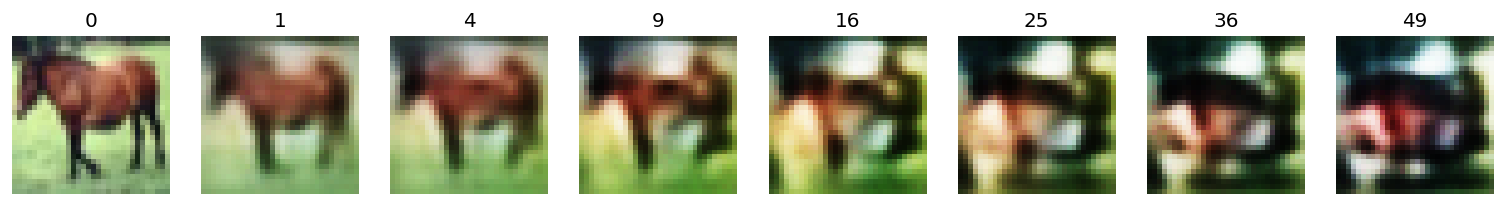
\includegraphics[width=\linewidth]{bootstrap/logan-b_1.png}
    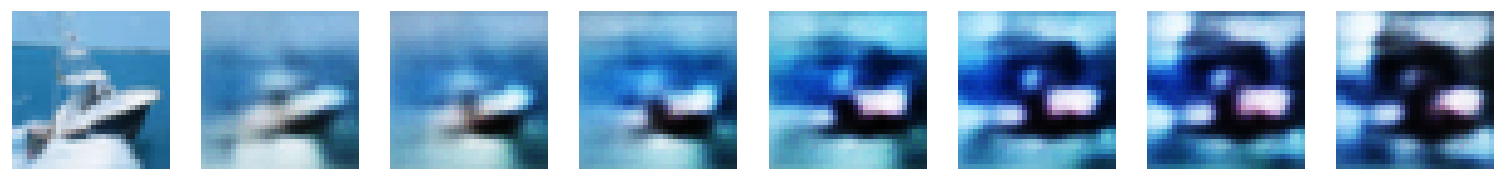
\includegraphics[width=\linewidth]{bootstrap/logan-b_2.png}
    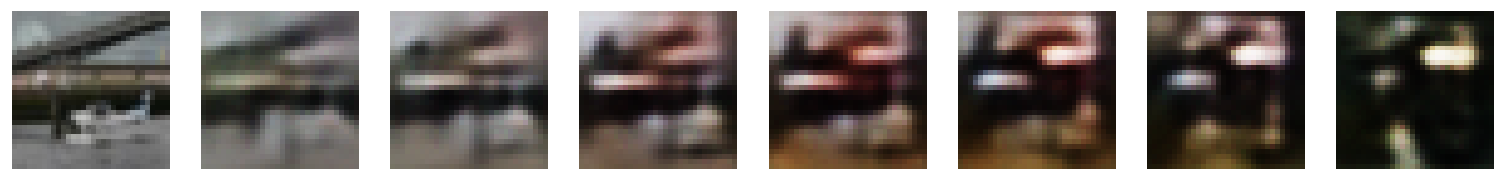
\includegraphics[width=\linewidth]{bootstrap/logan-b_3.png}
    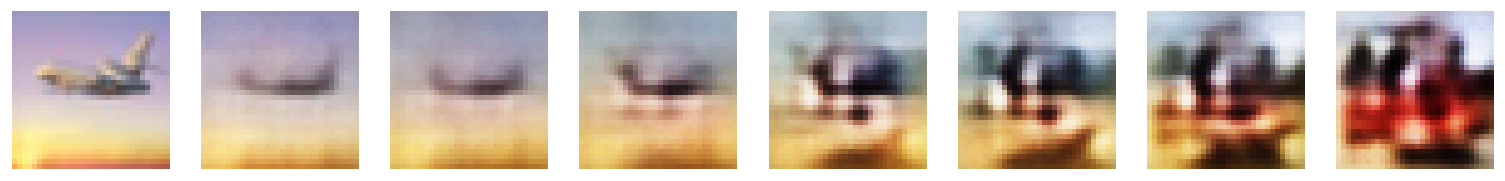
\includegraphics[width=\linewidth]{bootstrap/logan-b_4.png}
    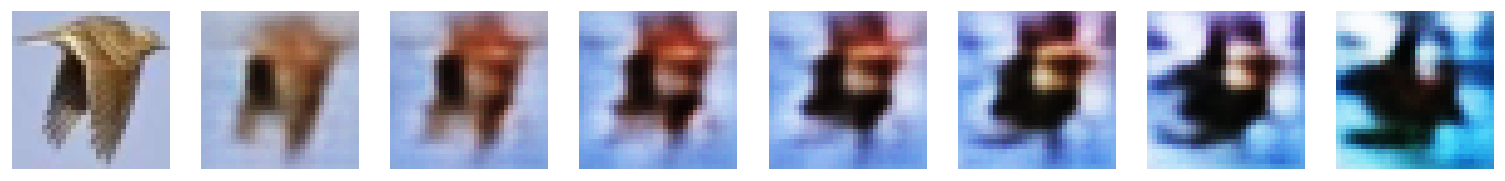
\includegraphics[width=\linewidth]{bootstrap/logan-b_5.png}
    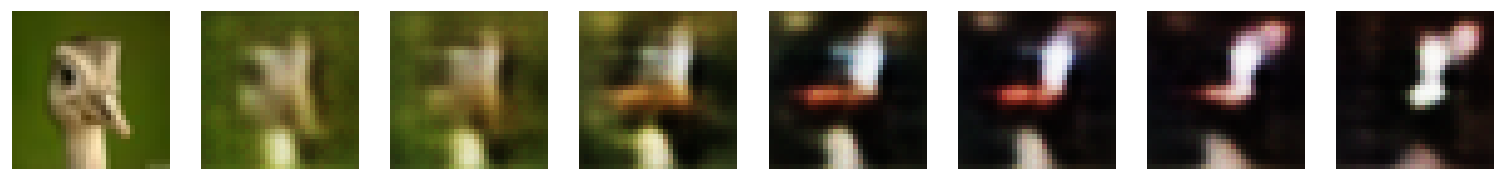
\includegraphics[width=\linewidth]{bootstrap/logan-b_6.png}
    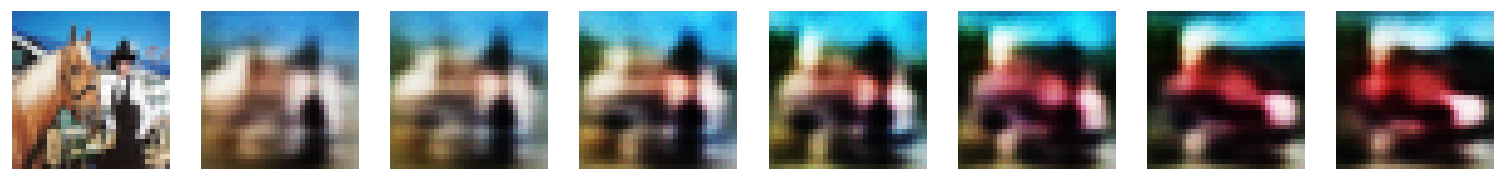
\includegraphics[width=\linewidth]{bootstrap/logan-b_7.png}
    \caption{Bootstrapping results on the CIFAR10 dataset. The first column contains the original images from the dataset. The number of bootstraps increases from left-to-right and is indicated at the top.}
    \label{fig:bootstrap_results}
\end{figure*}
\subsection{Bootstrapping}

One way to qualitatively visualize the reconstruction loss is by \textit{bootstrapping}: sampling from the training data, passing through the encoder and then passing the latent embedding again through the generator. The results from performing this on CIFAR10 are shown in Figure \ref{fig:bootstrap_results}. Interestingly, the last few columns seem to not change despite the number of bootstraps growing exponentially.


\section{Discussion}

The results indicate that the BiGAN training is the least stable of the three models that we considered. This instability is most likely caused by a lack of proper hyper-parameters. In practice, it can be expensive to tune hyperparameters when the space of hyperparameters that work is small. This is an additional weakness of the BiGAN model.
We have introduced a form of latent optimization for a bidirectional GAN (LOGAN-B) and shown improved ability to capture the space of the true distribution. We have also shown that the generator in the LOGAN-B framework can be more easily inverted due to the latent optimization provided by real training data.
A limitation to this work is that we only considered L1 loss for reconstruction. This type of loss is unlikely to scale for larger natural image datasets. Future work in this area should keep that in mind.

{\small
\bibliographystyle{ieee_fullname}
\bibliography{references}
}

\end{document}
